%!TEX root = FreeRtos ARM uController.tex
%\pagebreak
\subsection{Memory Allocation}
Beim Erzeugen von RTOS Objekten wie Tasks, Queues oder Semaphore wird Speicher im RAM benötigt. Für die dynamische Speicherverwaltung werden in C und C++ ge\-wöhnlich die Standard C-Funktionen malloc() und free() verwendet. Die Funktion malloc() dient zur Allokation von freiem Speicher und free() zur Freigabe von alloziertem Speicher. Für Echtzeitsysteme, die auf einem RTOS aufsetzen, sind diese Funktionen aufgrund der folgenden Eigenschaften\cite{MasteringFreeRtos} ungeeignet\footnote{Heap3 stellt hier eine Ausnahme dar}:
\needspace{3\baselineskip}
\begin{itemize}
	\item nicht thread safe
	\item nicht deterministisch
	\item tendieren zur Fragmentierung des RAM
	\item schwer zu debuggen
	\item Bibliotheksfunktionen benötigen viel Speicher
\end{itemize}
Des Weiteren sind für einige Einsatzgebiete von embedded Anwendungen Zertifikate erforderlich.\newline Speziell in sicherheitskritischen Anwendungen (z.B. Medical, Military) ist die dynamische Speicherverwaltung als eine potentielle Fehlerquelle auszuschließen. Für einen solchen Fall bietet FreeRTOS ab Version 9.0 die Möglichkeit der statischen Speicherallokation. Diese wird am Ende des Abschnitts betrachtet. In FreeRTOS werden malloc() und free() durch die Funktionen  
\begin{lstlisting}[label=lst:vPortMalloc1, numbers = none]
void *pvPortMalloc( size_t xSize );
\end{lstlisting}
und
\begin{lstlisting}[label=lst:vPortFree1, numbers = none]
void vPortFree( void *pv );
\end{lstlisting}
ersetzt. Dies hat den Vorteil, dass die Implementierung dieser Funktionen an die jeweilige Anwendung angepasst werden kann. FreeRTOS stellt dem Entwickler fünf unterschiedliche Implementierungen von Speicheralgorithmen (Heap\_1.c bis Heap\_5.c) zur Verfügung (siehe Abbildung \ref{fig:HeapsEclipse}). 
\begin{figure}[htb]
	\centering
		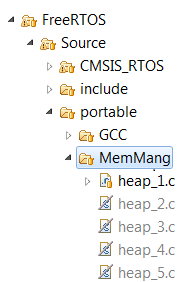
\includegraphics[width=0.2\textwidth]{Pictures/Eclipse/Heaps.png}
	\caption{Einbindung des Speicheralgorithmus Heap1 in Eclipse CDT. Die Algortihmen Heap2 bis Heap5 sind vom Build ausgeschlossen.}
	\label{fig:HeapsEclipse}
\end{figure}
\begin{lstlisting}[caption={FreeRTOS Source von pvPortMalloc() aus Heap1.c. Zuerst wird sichergestellt, dass die Startspeicheradresse dem byte-Alignment des $\mu$\-Pro\-zesso\-rs entspricht. Der STM32F4 ist ein 32Bit $\mu$\-Pro\-zesso\-r und hat ein byte-Alignment von 4, sodass die Startadresse immer eine Potenz von 4 sein muss. Danach wird der Scheduler deaktiviert und geprüft, ob genug Speicher zur Verfügung steht. Abschließend wird der Speicher im ucHeap reserviert.  }, linewidth=8cm,captionpos=b, label=lst:malloc2, float=htb]
void *pvPortMalloc( size_t xWantedSize )
{
void *pvReturn = NULL;
static uint8_t *pucAlignedHeap = NULL;
	#if( portBYTE_ALIGNMENT != 1 ){
		if( xWantedSize & portBYTE_ALIGNMENT_MASK )	{
			/* Byte alignment required. */
			xWantedSize += ( portBYTE_ALIGNMENT - ( xWantedSize & portBYTE_ALIGNMENT_MASK ) );
		}
	}
	#endif
	vTaskSuspendAll();
	if( pucAlignedHeap == NULL ){
		pucAlignedHeap = ( uint8_t * ) ( ( ( portPOINTER_SIZE_TYPE ) &ucHeap[ portBYTE_ALIGNMENT ] ) & ( ~( ( portPOINTER_SIZE_TYPE ) portBYTE_ALIGNMENT_MASK ) ) );
	}
	/* Check there is enough room left for the allocation. */
	if( ( ( xNextFreeByte + xWantedSize ) < configADJUSTED_HEAP_SIZE ) &&
		( ( xNextFreeByte + xWantedSize ) > xNextFreeByte )	)	{
		pvReturn = pucAlignedHeap + xNextFreeByte;
		xNextFreeByte += xWantedSize;
	}
	xTaskResumeAll();
	return pvReturn;
}
\end{lstlisting}
\begin{lstlisting}[caption={FreeRTOS Source von vPortFree() aus Heap1.c . Da eine Speicherfreigabe in Heap1 nicht vorgesehen ist, ist diese Funktion leer.}, linewidth=8cm,captionpos=b, label=lst:free2, float=htb]
void vPortFree( void *pv )
{
	/* Memory cannot be freed using this scheme. */
	( void ) pv;
	configASSERT( pv == NULL );
}
\end{lstlisting} 
Diese stellen prinzipiell schon die ge\-läu\-figsten Implementierungen zur Speicherverwaltung dar. Es bleibt aber auch weiterhin die Möglichkeit eine eigene Speicherverwaltung zu implementieren. In dieser Arbeit werden wir Heap1 genauer betrachten, um ein grund\-sätz\-liches Verständnis für die FreeRTOS Speicherverwaltung zu bekommen. Heap2 - Heap 5 werden nur kurz beschrieben und können im Detail in \cite{MasteringFreeRtos} und \cite{FreeRtosAdvanced} nachgelesen werden. Wie bereits am Anfang dieses Abschnitts beschrieben, wird für alle RTOS Objekte Speicher benötigt. Der Speicher für Objekte wie Semaphore und Tasks wird automatisch in den statischen Erzeugerfunktionen der RTOS API alloziert, indem intern die Funktion \textit{pvPortMalloc()} aufgerufen wird. Die Erzeugerfunktion xTaskCreate() beispielsweise erzeugt einen FreeRTOS Task. Listing \ref{lst:xTaskCreate} zeigt wie xTaskCreate() die Funktion pvPortMalloc() verwendet, um Speicher für den Stack und den Task Control Block zu allozieren.
\begin{lstlisting}[caption={FreeRTOS Source von xTaskCreate() aus Task.c. Jeder Task besitzt einen Stack und einen Task Control Block, beide werden beim Aufruf von xTaskCreate (Zeile 5 und Zeile 11) erstellt.}, linewidth=8cm,captionpos=b, label=lst:xTaskCreate, float=htb]
StackType_t *pxStack;
pxStack = ( StackType_t * ) pvPortMalloc(( ( ( size_t ) usStackDepth ) 
* sizeof( StackType_t ) ) );
if( pxStack != NULL )
{
	pxNewTCB = ( TCB_t * ) pvPortMalloc( sizeof( TCB_t ) );
	if( pxNewTCB != NULL )
	{
		pxNewTCB->pxStack = pxStack;
	}

}
\end{lstlisting}
Alle Objekte, die mittels pvPortMalloc() alloziert werden, darunter auch der Kernel selbst, teilen sich einen gemeinsamen Adressraum (siehe Abbildung \ref{fig:AddressSpace}). 
\begin{figure}[hbt]
	\centering
		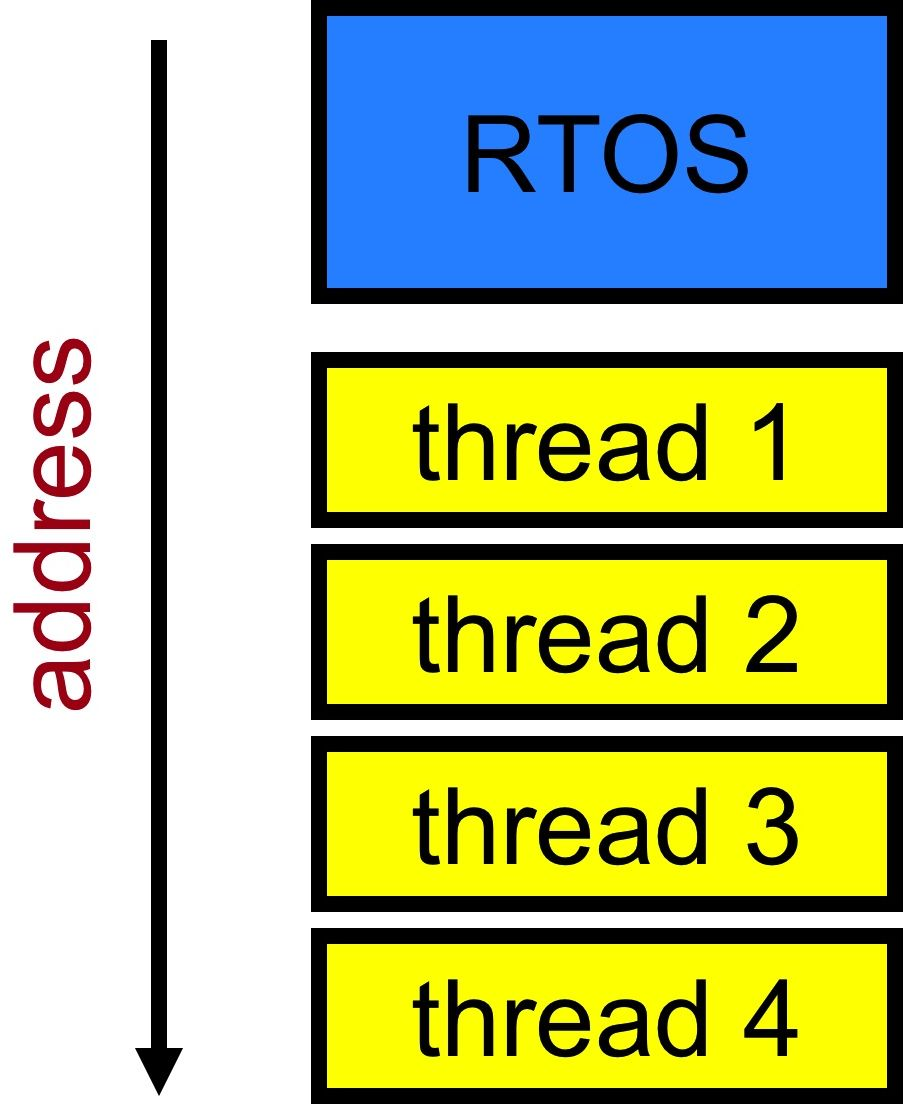
\includegraphics[width=0.2\textwidth]{Pictures/EmbeddedCom/addressSpace.jpg}
	\caption{Task und Kernel teilen sich in FreeRTOS einen gemeinsamen Adressraum. Dies stellt eine potentielle Fehlerquelle dar. Bild-Quelle~\protect\citeA{RTOSRevealed}}
	\label{fig:AddressSpace}
\end{figure} 
Durch den gemeinsamen Adressraum ist es beispielsweise mög\-lich, dass durch einen Überlauf oder einem ungewollten Speicherzugriff, Daten eines anderen Tasks oder des Kernels ver\-än\-dert werden.   
%Christoph: Ein ungewollter Speicherzugriff ist somit durchaus möglich. Durch die Umschreibung des vorherhigen Satzes jetzt doppelt.
%Christoph:Durch den gemeinsamen Adressraum ist es bei fehlerhaften Verwendungen von Speicherzugriffsfunktionen möglich aus einer Task auf die Variablen einer anderen Task zuzugreifen. 
%Michael: Ich habe das nochmal umformuliert. Es ist nicht durch die fehlerhafte Verwendung möglich auf Variablen einer anderen Task zuzugreifen. Das ist grundsätzlich möglich und auch gewollt.  
In Abschnitt \ref{sec:Memory Protection} wird gezeigt welche Mög\-lich\-keit der STM32F4 und FreeRTOS bieten um Speicherzugriffe sicherer zu gestalten.    
%\pagebreak 
%\cleardoublepage
%\FloatBarrier
\subsubsection{FreeRTOS Algorithmen zur Speicherverwaltung}
Bevor Objekte erzeugt werden können, muss ein Pool an Speicher für die Objekte definiert werden. Die einfachste Form, einen Memory Pool zu erzeugen, ist ein Array. In FreeRTOS nennt sich dieses Array ucHeap:
\begin{lstlisting}[numbers = none]
static uint8_t ucHeap[ configTOTAL_HEAP_SIZE ];
\end{lstlisting}
Die Größe des Heaps wird durch das Prä\-pro\-zes\-sor-Define configTOTAL\_HEAP\_SIZE (FreeRTOS\_config.h) konfiguriert. Die Gesamtgröße berechnet sich wie folgt:
\newline
\newline
MaxHeapSize $=$ configTOTAL\_HEAP\_SIZE $\ast$ Wortbreite\footnote{Beim STM32F4 ist die Wortbreite 32 bit} 
\newline
\newline
Die Speicherverwaltung durch Heap1 ist sehr einfach.\newline 
Heap1 deklariert die Funktion pvPortMalloc(). Die Funktion pvPortFree() wird nicht ausimplementiert. Abbildung \ref{fig:Heap1} zeigt wie der Speicher nach dem Erzeugen von zwei Tasks aussieht. 
\begin{figure}[htb]
	\centering
		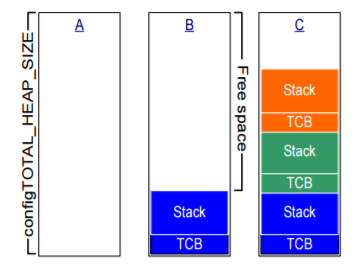
\includegraphics[width=0.3\textwidth]{Pictures/FreeRTOSOrg/heap1Alg.png}
	\caption{Beispiel Speicherbelegung nach drei Instanziierungen von Tasks durch die Erzeugerfunktion xTaskCreate() unter Verwendung des Speicheralgorithmus Heap1. Bild-Quelle~\protect\citeA{MasteringFreeRtos}}
	\label{fig:Heap1}
\end{figure}
Für jeden Task wird ein TCB und ein Stack erzeugt. Die Speicherobjekte liegen direkt hintereinander. Da pvPortFree() nicht implementiert ist und in der Folge allozierter Speicher nicht freigegeben werden kann, kommt es nicht zu einer Fragmentierung des Speichers. Diese lineare Speicherzuweisung gilt für alle Objekte, die mittels pvPortMalloc() alloziert werden. Dazu gehören sowohl RTOS spezifische Objekte, als auch Objekte, die durch den Entwickler erzeugt werden. Ein so einfacher Speicheralgorithmus wie Heap1 hat seine Berechtigung. Bei vielen embedded Anwendungen wird der Speicher für die benötigten Objekte vor dem Start des Schedulers erzeugt. Eine spätere Freigabe von belegten Ressourcen ist nicht nötig, da die Objekte über die gesamte Laufzeit des Programms bestehen sollen. Für solche Anwendungen steht Heap1 zur Verfügung. Nachfolgend ein Kurz\-über\-blick über die nicht beschriebenen Speicheralgorithmen:  
\begin{itemize}
	\item Heap2 - Ähnlicher Algorithmus wie Heap1. Erlaubt allerdings Speicherfreigabe durch vPortFree(). Best Fit Algorithmus zur Speicherallokation. 
	\item Heap3 - Verwendet C Library Malloc() und free() und deaktiviert den Scheduler zur Speicherallokation.
	\item Heap4 - Ähnlicher Algorithmus wie Heap1 und Heap2. Verwendet First Fit Algorithmus zur Speicherallokation. Verbindet mehrere kleinere Speicherblöcke zu einem Großen. Minimiert Speicherfragmentierung.
	\item Heap5 - Gleicher Algorithmus wie Heap4. Es kön\-nen mehrere Memory Pools erzeugt werden.
	%Christoph: Ich habe versucht die Aufzählung etwas zu vereinheitlichen. Ggf. muss du noch etwas nachsteuern
	%Michael: Okay :)
\end{itemize}
\subsubsection{Memory Protection}
\label{sec:Memory Protection}
Embedded Softwaresysteme können durch den Einsatz einer Memory Protection Unit (MPU) eine weitere Steigerung der Zuverlässigkeit erreichen. Die MPU bietet eine hardwarebasierte Lösung zur Detektion von ungewollten Speicherzugriffen (Abbildung \ref{fig:AddressSpaceMMU}). 
\begin{figure}[htb]
	\centering
		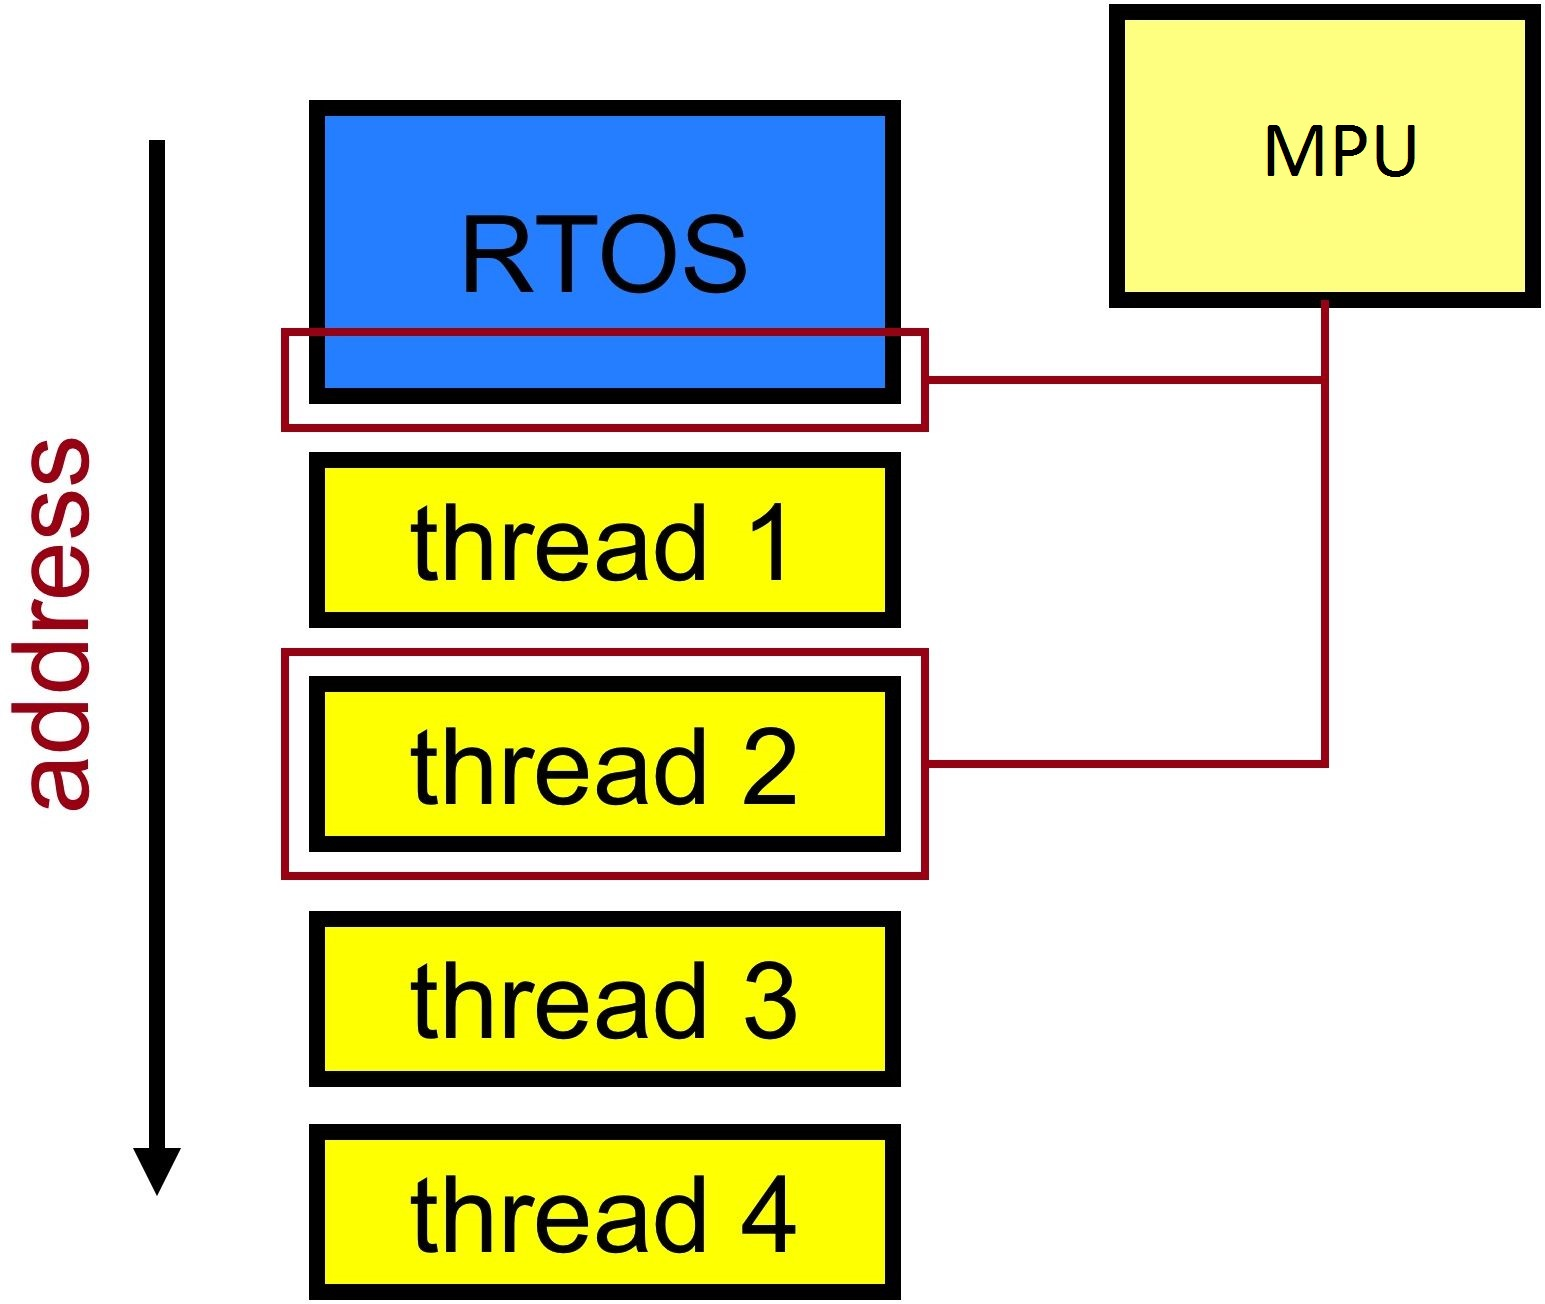
\includegraphics[width=0.3\textwidth]{Pictures/EmbeddedCom/addressSpaceMMU}
	\caption{Zugriffsrechte für einen Restricted Task werden durch den RTOS Kernel in der MPU konfiguriert. Der Speicherzugriff wird automatisch durch MPU überprüft und im Fehlerfall an den Kernel gemeldet. Bild-Quelle~\protect\citeA{RTOSRevealed}}
	\label{fig:AddressSpaceMMU}
\end{figure} 
Für die MPU des STM32F4 $\mu$\-Pro\-zesso\-rs steht eine spezielle API Portierung von FreeRTOS zur Verfügung (FreeRTOS-MPU). Zur Erzeugung von Tasks, die die MPU nutzen sollen, muss die Erzeugerfunktion xTaskCreateRestricted() verwendet werden. Beim Aufruf der Erzeugerfunktion wird dem Kernel die Stackadresse des Tasks mitgeteilt, damit dieser die entsprechenden Zugriffsberechtigungen der Speicheradressen konfigurieren kann. Die so erzeugten Tasks werden Restricted Tasks genannt. Der Zugriff aus einem Restricted Task auf den Speicher (Task-Stack) eines anderen Restricted Tasks ist nicht erlaubt. Bei einem nicht erlaubten Speicherzugriff wird automatisch die entsprechende Hook-Funktion aufgerufen. Dem System wird so ermöglicht, entsprechend zu reagieren. Restricted Tasks kön\-nen sich in einem der folgenden Modi befinden:
\begin{itemize}
	\item User Mode
	\item Privileged Mode 
\end{itemize}
Im User Mode ist es einem Restricted Task nicht erlaubt auf den Speicher des FreeRTOS Kernels zuzugreifen. So wird verhindert, dass der Kernel ungewollt modifiziert wird. Nur einem Restricted Task, der sich im Privileged Mode befindet, ist ein Zugriff auf den Kernel Speicher erlaubt. Dabei geschieht der Wechsel vom User Mode in den Privileged Mode implizit durch den Aufruf einer FreeRTOS API Funktion. Ein Wechsel durch den Task selbst in den Privileged Mode ist nicht möglich.
\subsubsection{Static Memory Allocation}
Die statische Speicherverwaltung wird durch das Prä\-pro\-zes\-sor-Define configSUPPORT\_STATIC\_ALLOCATION 1 in der FreeRTOS\_config aktiviert. Für die statische Objekterzeugung können die dynamischen Erzeugerfunktionen nicht mehr verwendet werden, daher stehen spezielle Erzeugerfunktionen für die statische Speicherallozierung zur Verfügung. Beispiele hierfür sind: xTaskCreateStatic() statt xTaskCreate() oder xSemaphoreCreateBinaryStatic() statt xSemaphoreCreateBinary(). Der Vorteil der statischen Speicherverwaltung ist, dass der belegte Speicher im RAM schon zur Übersetzungszeit bekannt ist und die potenzielle Fehlerquelle der dynamischen Speicherverwaltung vermieden wird. Der Nachteil besteht darin, dass mehr RAM verwendet wird, als bei den meisten Heap Implementierungen. Heap1 stellt eine geeignete Alternative in der dynamischen Speicherverwaltung dar, da es die Risiken der dynamischen Speicherverwaltung auf ein Minimum reduziert.   
Die statische Speicherverwaltung wird durch das Prä\-pro\-zes\-sor-Define configSUPPORT\_STATIC\_ALLOCATION 1 in der FreeRTOS\_config aktiviert. Für die statische Objekterzeugung können die dynamischen Erzeugerfunktionen nicht mehr verwendet werden. Daher stehen spezielle Erzeugerfunktionen für die statische Speicherallokation zur Verfügung. Beispiele hierfür sind: 
\begin{itemize}
	\item xTaskCreateStatic() statt xTaskCreate()
	\item xSemaphoreCreateBinaryStatic() statt xSemaphoreCreateBinary()
\end{itemize}
Der Vorteil der statischen Speicherverwaltung ist, dass der belegte Speicher im RAM schon zur Übersetzungszeit bekannt ist und die potenzielle Fehlerquelle der dynamischen Speicherverwaltung vermieden wird. Der Nachteil besteht darin, dass mehr RAM verwendet wird, als bei den meisten Heap Implementierungen. Heap1 stellt eine geeignete Alternative in der dynamischen Speicherverwaltung dar, da es die Risiken der dynamischen Speicherverwaltung auf ein Minimum reduziert.   